\documentclass[a4paper]{article}
\usepackage[utf8]{inputenc}
\usepackage{amsmath}
\usepackage{amssymb}
\usepackage{amsfonts}
\usepackage{amsthm}
\usepackage{tikz}

\title{Homework 1}
\author{Vanja Stojanović}
\date{March 2025}

\begin{document}

\maketitle

\section{Time Complexity}
We analyse within the RAM model, and assign a cost $c_k$ to the $k$-th instruction. 

\subsection{Exercise - function \texttt{t1}}
We assume a \texttt{for} loop will check the condition and execute its operation in one cycle. 
Let $T_{t1}(n)$ be the running-time complexity of the function \texttt{t1} with the input of size $n$. Then we have the following

\[
    T_{t1}(n) = c_1 + c_2 \sum_{i=1}^{n+1}t_i + c_3 \sum_{i=1}^{n}t_i + c_4
\]

\noindent
where $t_i = 1$ is the number of times the inner \texttt{for}. We can expand to

\begin{align*}
    T_{t1}(n) &= c_1 + c_2 (n + 1) + c_3n + c_4\\
    &=  n(c_2 + c_3) + c_1 + c_2 + c_4
\end{align*}

\noindent
we conclude that $T_{t1}(n) = O(n)$.

\subsection{Exercise - function \texttt{t2}}

We assume a more strict RAM, where each part of the \texttt{for} loop counts as one instruction.
Let $T_{t2}(n)$ be the running-time complexity of the function \texttt{t2} with the input of size $n$. Then we have the following

\begin{align*}
    T_{t2}(n) &= c_1 + \underbrace{c_2 + c_3 (n+1) + c_4 n}_{\texttt{for}_1} \\
    &+ \underbrace{\sum_{i = 1}^{n}(c_4 + c_5 (\log_2 (i) + 1) + c_6 \log_2(i)+ \sum_{i}^{log_2(i)} T_{t1}(i))}_{\texttt{for}_2}  +\ c_7
\end{align*}

\noindent
we conclude that $T_{t2}(n)=O(n^2\log n)$, since the first loop will runn $n$ times and the second loop will loop $log_2(i) \cdot i$ times ($i$ gets to $n$ in the last iteration).

\subsection{Exercise - function \texttt{cantor}}
Let $T_{cantor}$ be the running-time complexity of the function \texttt{cantor}. Since the function is recursive we can use Master's theorem
to analyse its time complexity. It states that

\begin{equation*}
    T(n) = \left \{ 
        \begin{array}{lc}
            \Theta (n^k)&;\ a < b^k\\
            \Theta (n^k \log n)&; a = a^k\\
            \Theta (n^{\log_b a})&; a > b^k
        \end{array}
    \right .    
\end{equation*}

\noindent
where  the time complexity is of the following form

\label{eq_master}
\begin{equation}
    T(n) = aT(\frac n b) + cn^k
\end{equation}

We define $a$ as the number of recursive calls, in this case $a = 2$, $b$ as the factor by which the problem size is divided, in this case $b=2$, and
$k$ as the exponent of the non-recursive work, which in this case is linear (or non-dependant of $n$) so $k = 0$. We substitute the values into equation
\ref{eq_master} and derive the following

\begin{equation}
    T_{cantor} (n) = 2T(\frac n 2) + cn^0
\end{equation}

Since this is the condition where $a > b^k$, we conclude that $T_{cantor} (n) = \Theta (n^{\log_2 2}) = \Theta(n)$.

\section{Generating Functions}

\subsection{Exercise 4}

We seek to find the number of distinct nonnegative integer solutions to the following equation

\label{naloga4}
\begin{equation}
    x_1 + 2x_2 + 5x_3 + 10x_4 = 13
\end{equation}

\noindent
We define a family of generating functions $G_n(x)$ where $n$ represents the leading factor of the terms above as

\[
    G_n(x) = 1 + x^n + x^{2n} + x^{3n} + ...
\]

\noindent
Since for $|x| < 1$ the geometric series converges as follows

\[
    \sum_{n = 0}^{\infty} ax^n = \frac{a}{1 - x}
\]

\noindent
with our common factor we can reduce the generating functions to

\[
    G_n(x) = \frac{1}{1 - x^n}
\]

\noindent
We then calculate the number of solutions by multiplying the functions $G_1(x)$, $G_2(x)$, $G_5(x)$, $G_{10}(x)$ as shown below
\newpage

\begin{align*}
    G_1(x)G_2(x)G_5(x)G_{10}(x) &= (1 + x + x^{2} + x^{3} + ...)\\
                                &\quad\cdot\ (1 + x^2 + x^{4} + x^{6} + ...)\\
                                &\quad\cdot\ (1 + x^5 + x^{10} + x^{15} + ...)\\
                                &\quad\cdot\ (1 + x^10 + x^{20} + x^{30} + ...)\\
                                &= 1 + x + 2 x^2 + 2 x^3 + 3 x^4 + 4 x^5+ 5 x^6 + 6 x^7 + 7 x^8  \\
                                &\quad +\ 8 x^9  + 11 x^{10} + 12 x^{11}+ 15 x^{12} + 16 x^{13} +...
\end{align*}

We take the coefficient of the term $x^{13}$ and conclude that there are 16 nonnegative integer solutions to equation \ref{naloga4}. The next equation for
which we seek the number of distinct nonnegative integer solutions is 

\label{naloga4_2}
\begin{equation}
    x_1 + 2x_2 = 13
\end{equation}

\noindent
We again multiply our generating functions, now only $G_1(x)$, $G_2(x)$

\begin{align*}
    G_1(x)G_2(x)&= (1 + x + x^{2} + x^{3} + ...)\\
                &\quad\cdot\ (1 + x^2 + x^{4} + x^{6} + ...)\\
                &= 1 + x + 2 x^2 + 2 x^3 + 3 x^4 + 3 x^5+ 4 x^6 + 4 x^7 + 5 x^8  \\
                &\quad +\ 5 x^9  + 6 x^{10} + 6 x^{11}+ 7 x^{12} + 7 x^{13} +...
\end{align*}

We again take the coefficient of the term $x^{13}$ and conclude that there are 7 nonnegative integer solutions to equation \ref{naloga4_2}.
\begin{flalign*}
    &&  && \blacksquare
\end{flalign*}

\subsection{Exercise 5}

A triangle number $n$ is a number of the form 

\[
    T_n = \sum_{i=1}^{n}i = \frac{n(n+1)}{2}
\]

\noindent
We derive the generating function $G(x)$ by starting with the geometric series

\[
\frac{1}{1-x} = \sum_{n=0}^{\infty} x^n
\]

\noindent
we differentiate

\[
\frac{1}{(1-x)^2} = \sum_{n=0}^{\infty} nx^{n-1} = \sum_{n=1}^{\infty} n x^{n-1} =\sum_{n=0}^{\infty} (n+1)x^{n}
\]

\noindent
and we differentiate again

\[
\frac{2}{(1-x)^3} = \sum_{n=0}^{\infty} n(n+1)x^{n-1} = 2 \sum_{n=0}^{\infty} T_nx^{n-1} = 2 \sum_{n=1}^{\infty} T_nx^{n-1} = 2 \sum_{n=0}^{\infty} T_{n+1}x^{n}
\]

\newpage
\noindent
thus

\[
    G(x) = \sum_{n=0}^{\infty} T_{n+1}x^{n} = \frac{1}{(1- x)^3}
\]

Then calculating the 100th triangular number equates to finding the coefficient of the term where the exponent is $100$. We input $n = 99$

\[
    G(x) = x + 3x^2 + 6x^3 + ... + 5050 x^{100} +...
\]

\noindent
concluding that the 100th triangular number is $5050$.
\begin{flalign*}
    &&  && \blacksquare
\end{flalign*}


\subsection{Exercise 6}

We wish to show, that every positive integer can be written in exactly one way as the sum of distinct powers of 2. We can derive a generating function
to show that we can either choose an exponent or no as follows

\[
G(x) = (1+ x^{2^0})(1+ x^{2^1})(1+ x^{2^2})(1+ x^{2^3})\cdots = \prod_{k = 0}^{\infty} (1 + x^{2^i})
\]

\noindent
when expanding this product each factor $(1 + x^{2^i})$ contributes either $1$ or $x^{2^i}$. Therefore, any monomial in the expansion is of the form

\[
x^{\epsilon_0 \cdot 2^0 + \epsilon_1 \cdot 2^1 + \epsilon_2 \cdot 2^2+ \cdots}
\]

\noindent
with each $\epsilon_i \in \{0,1\}$. The exponent is exactly the sum of a subset of distinct powers if 2. Notice that every nonnegative integer has a unique binary expansion. In other words,
for every nonnegative integer $n$ there exists a unique sequence $(\epsilon_0, \epsilon_1, \epsilon_2,...)$ with $\epsilon_i \in \{0,1\}$ such that

\[
n = \epsilon_0 \cdot 2^0 + \epsilon_1 \cdot 2^1 + \epsilon_2 \cdot 2^2+ \cdots
\]

Thus, in the generating function $G(x)$ the monomial $x^n$ appears exactly once since there is only one way to form $n$ as a sum of distinct powers of $2$.

\begin{flalign*}
    &&  && \blacksquare
\end{flalign*}

\newpage
\section{Turing Machines}

\subsection{Exercise 7}

The Turing machine checks that there is a corresponding letter from the input alphabet on the other side of the given sequence, yielding a guarrantee
for a palindrome. Once the tape is completely blank we are finished, or when there are no defined transitions then the sequence was not a palindrome.

\begin{figure}[ht!]
    \centering
    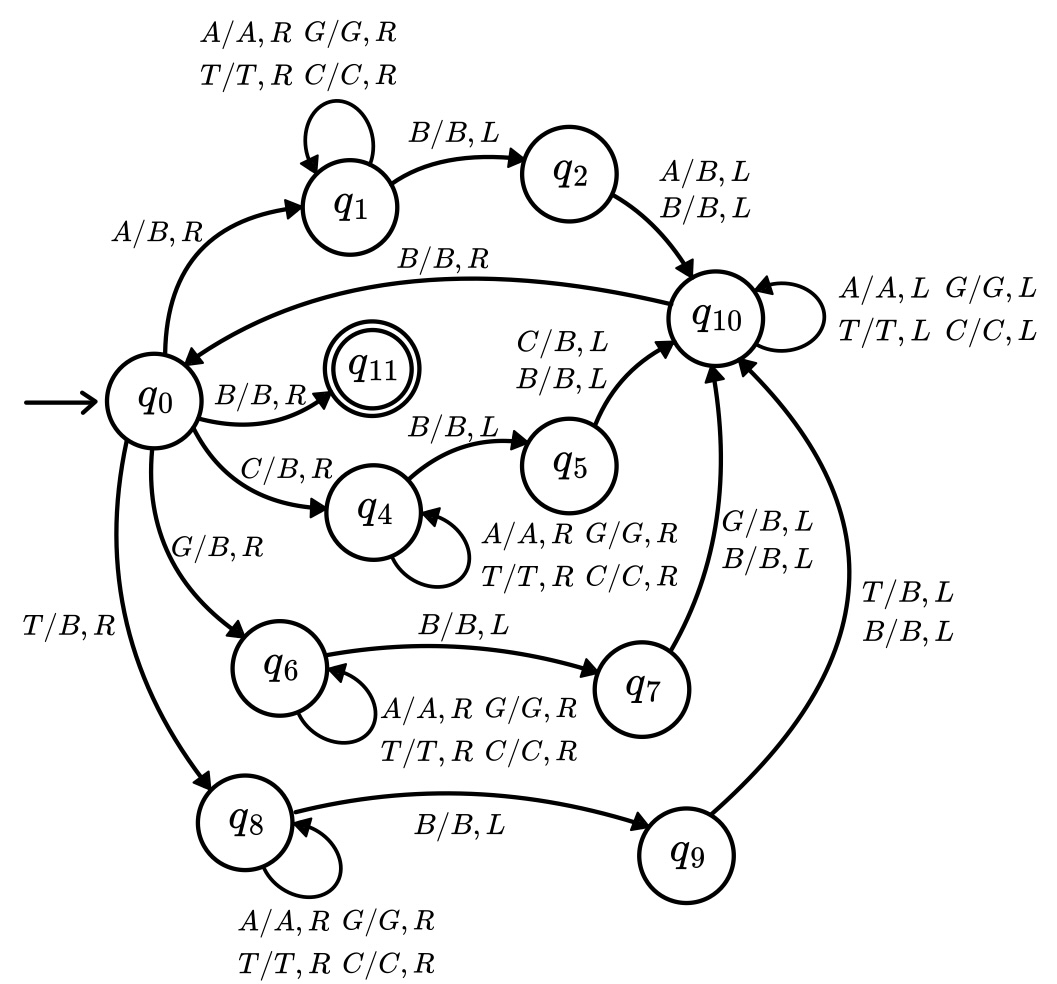
\includegraphics[scale = 0.3]{assets/Turing-1.jpeg}
    \caption{Turing machine for exercise 7}
\end{figure}

\newpage
\subsection{Exercise 8}

The Turing machine first checks for unmatched parenthesis, if found it marks it with a $\#$ symbol, then it searches for a closing one, again marking
it with a $\#$. It repeats this for the entire sequence.

\begin{figure}[ht!]
    \centering
    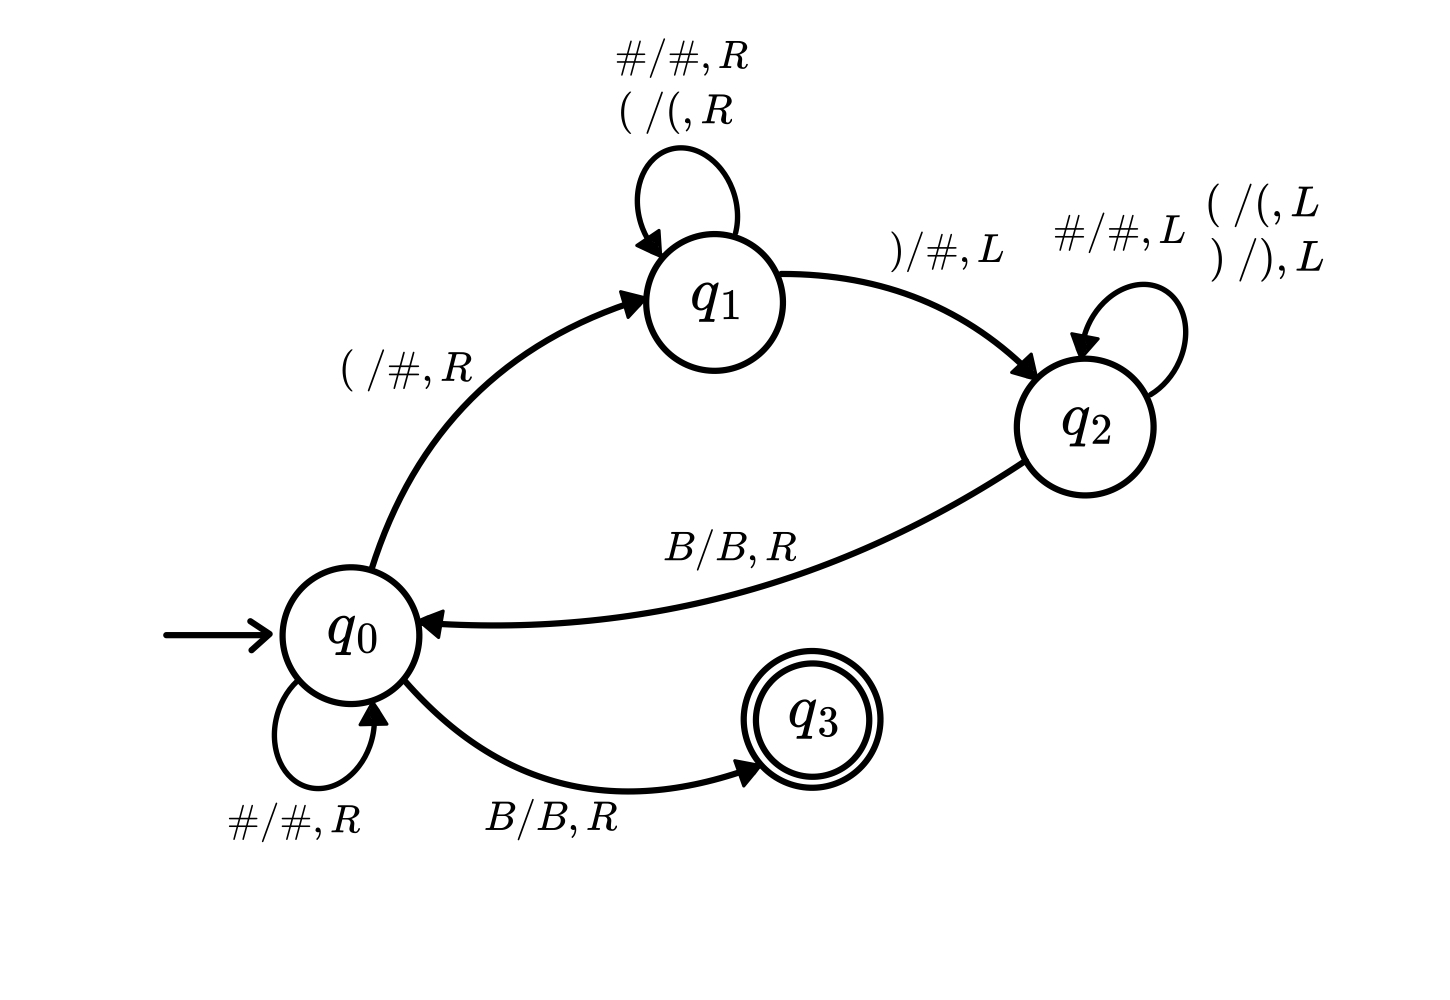
\includegraphics[scale = 0.2]{assets/Turing-2.jpeg}
    \caption{Turing machine for exercise 8}
\end{figure}

\subsection{Exercise 9}

The Turing machine marks the first unmatched symbol in the first half of $w$ with $X$, then searches for an unmatched symbol in the second half of 
$w$ and mark it with $Y$. It repeats this until the concatination gets checked and completely marked. The Turing machine can be seen below, on the next
page.
\newpage

\begin{figure}[ht!]
    \centering
    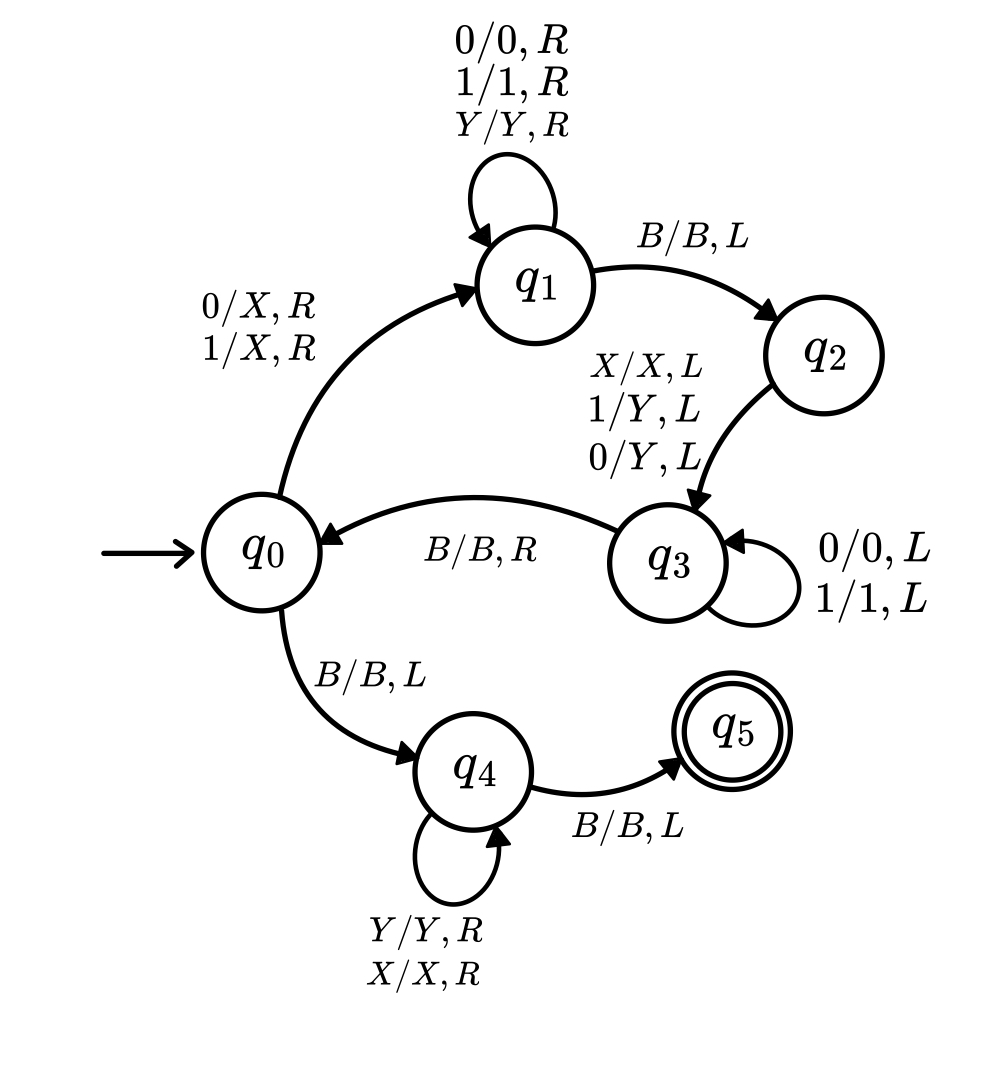
\includegraphics[scale = 0.25]{assets/Turing-3.jpeg}
    \caption{Turing machine for exercise 9}
\end{figure}

\end{document}

